\section{Introduction}

Redundant Arrays of Independent Disks (RAID) is a storage technology introduced in the 1980s by Patterson. 
Its purpose is to enhance the performance, capacity, and reliability of storage systems. 
RAID achieves this by combining multiple independent disks into a single logical unit with improved performance.

This approach stands in contrast to Just a Bunch of Disks (JBOD), where each disk functions as a separate entity with its own mount point.
Instead, RAID stripes data across several disks, allowing for parallel access. 
This striping enables high data transfer rates for large data accesses and high I/O rates for small, frequent data accesses.
Additionally, it facilitates load balancing across the disks.

RAID employs two primary techniques: data striping to boost performance and redundancy to enhance reliability. 
These orthogonal methods work together to provide improved storage capabilities for various computing needs.

The distribution of data in RAID systems is facilitated through I/O virtualization.
This means that data is distributed transparently across the disks, requiring no action from the users. 

\subsection{Data striping}
Data striping in RAID involves writing data sequentially, such as vectors, files, or tables, onto multiple disks in units called stripes. 
These stripes can be defined by various units, such as bits, bytes, or blocks, and are written according to a cyclic algorithm, typically a round-robin approach.

The stripe unit refers to the size of the data unit that is written on a single disk, while the stripe width indicates the number of disks considered by the striping algorithm.

There are several benefits to data striping:
\begin{itemize}
    \item Multiple independent I/O requests can be executed in parallel by several disks, reducing the queue length and overall response time of the disks.
    \item Single multiple-block I/O requests can be executed by multiple disks in parallel, increasing the transfer rate of individual requests.
\end{itemize}

Indeed, as the number of physical disks in a RAID array increases, so do the potential size and performance gains.
However, this also comes with a corresponding increase in the probability of failure of any one disk within the array. 
This heightened risk of disk failure underscores the importance of introducing redundancy into the system.

Redundancy in RAID serves as a safeguard against data loss in the event of disk failure. 
By duplicating or distributing data across multiple disks in a redundant manner, the system can withstand the failure of one or more disks without losing critical data. 
Redundancy mechanisms such as mirroring (RAID 1), parity (RAID 5), or both (RAID 6) provide fault tolerance and ensure data integrity even in the face of hardware failures.

\paragraph*{Performance}
In redundancy-based RAID configurations, error correcting codes are computed and stored on disks separate from those holding the primary data. 
These error correcting codes provide the ability to tolerate data loss resulting from disk failures. 
However, the implementation of redundancy introduces overhead in terms of performance, particularly during write operations.

During write operations, updates must also be made to the redundant information, which results in a performance penalty compared to traditional writes. 
This is because the additional computation and storage required for redundancy checking and updating the error correcting codes increase the time required to complete write operations.

\paragraph*{RAID}
Indeed, hard drives are invaluable storage devices, offering relatively fast and persistent storage. 
However, they have their shortcomings, primarily in terms of coping with disk failure and limited capacity.

To address these limitations, RAID (Redundant Array of Independent Disks) technology comes into play. 
RAID leverages multiple disks to create the illusion of a single, larger, faster, and more reliable disk.
Externally, RAID operates seamlessly, appearing as a single disk to users. 
This transparency means that data blocks are read and written just as they would be on a single disk, without the need for software to explicitly manage multiple disks or perform error checking and recovery tasks.

Internally, however, RAID is a sophisticated computer system. 
Disks are managed by dedicated CPUs and specialized software, with support from RAM and non-volatile memory. 
RAID offers a wide array of configuration options, known as RAID levels, each tailored to different needs and priorities, such as performance, redundancy, or a balance of both.

RAID offers various levels, each with its own method of data organization and redundancy. 
Here's an overview of the commonly known RAID levels:
\begin{enumerate}
    \item RAID 0: striping only. 
        Data is striped across multiple disks without redundancy. 
        This offers improved performance by spreading data across disks, but there's no fault tolerance, meaning if one disk fails, all data is lost.
    \item RAID 1: mirroring only. 
        Data is mirrored across pairs of disks. 
        This provides redundancy, as data is duplicated on each disk. 
        If one disk fails, data remains intact on the mirrored disk.
    \item RAID 0+1 (also known as RAID 01): a nested RAID level combining RAID 0 (striping) and RAID 1 (mirroring). 
        Data is striped across mirrored sets of disks. 
        This offers both performance benefits and redundancy.
    \item RAID 1+0 (also known as RAID 10): another nested RAID level combining RAID 1 (mirroring) and RAID 0 (striping). 
        Data is mirrored first and then striped across the mirrored sets. 
        This also provides both performance and redundancy.
    \item RAID 2: bit interleaving, which is not commonly used in practice.
    \item RAID 3: byte interleaving with dedicated parity disk. 
        Data is striped across disks, and parity information is stored on a dedicated disk for fault tolerance.
    \item RAID 4: block interleaving with dedicated parity disk. 
        Similar to RAID 3, but operates at the block level rather than the byte level.
    \item RAID 5: block interleaving with distributed parity blocks. 
        Data and parity information are striped across multiple disks, with parity blocks distributed among the disks. 
        This provides fault tolerance with improved performance compared to RAID 3 and 4.
    \item RAID 6: similar to RAID 5 but with greater redundancy. 
        It can tolerate the failure of up to two disks simultaneously, as it utilizes double parity to protect against data loss.
\end{enumerate}

\subsection{Performance}
\paragraph*{Sequential transfer rate}
We typically examine sequential and random workloads. 
Assuming disks in the array have a sequential transfer rate $S$:
\[S=\dfrac{\text{transfer size}}{\text{time to access}}\]
\begin{example}
    Consider a 10 megabyte transfer and a hard disk with the following characteristics:
    \begin{itemize}
        \item Average seek time of seven milliseconds.
        \item Average rotational delay of three milliseconds.
        \item Transfer rate of 50 megabytes per second.
    \end{itemize}
    The transfer rate in this case will be:
    \[S=\dfrac{10\:MB}{7\:ms+3\:ms+\frac{10\:MB}{50\:MB/s}}= 47.62\:MB/s\]
\end{example}

\paragraph*{Random transfer rate}
Again, we focus on sequential and random workloads. 
Assuming disks in the array have a random transfer rate $R$:
\[R=\dfrac{\text{transfer size}}{\text{time to access}}\]
\begin{example}
    Consider a 10 kilobyte transfer and a hard disk with the following characteristics:
    \begin{itemize}
        \item Average seek time of seven milliseconds.
        \item Average rotational delay of three milliseconds.
        \item Transfer rate of 50 megabytes per second.
    \end{itemize}
    The transfer rate in this case will be:
    \[S=\dfrac{10\:KB}{7\:ms+3\:ms+\frac{10\:MB}{50\:MB/s}}= 0.98\: MB/s\]
\end{example}

\subsection{Consistent update}
Mirrored writes should be atomic, meaning that all copies are written, or none are written.
However, this is difficult to guarantee. Many RAID controllers include a write-ahead log, which is a battery-backed, non-volatile storage of pending writes. 
A recovery procedure ensures that the out-of-sync mirrored copies are recovered.

\subsection{Main levels comparison}
\begin{figure}[H]
    \centering
    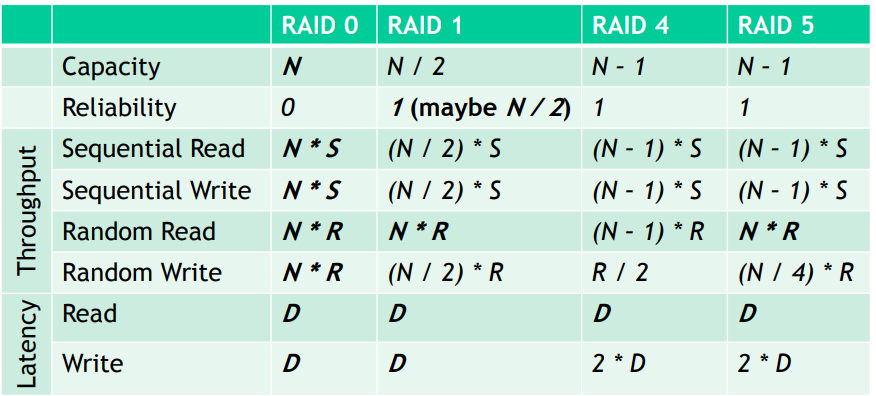
\includegraphics[width=0.6\linewidth]{images/levcomp.png}
    \caption{RAID levels comparison}
\end{figure}
Here, $N$ refers to the number of drives, $S$ represents sequential access speed, $R$ denotes random access speed, and $D$ signifies the latency required to access a single disk.